\section{Introduction} 
\label{sec:intro}

Visual \ac{SLAM} \cite{cadena2017past,ORBSLAM3_TRO,slam-handbook} is experiencing a paradigm shift toward dense mapping methods that generate accurate 3D maps in real time. Beyond traditional feature-based pipelines \cite{ORBSLAM3_TRO}, recent approaches leverage feed-forward dense pointmap estimators \cite{dust3r_cvpr24} as a front-end to directly reconstruct scenes while estimating camera poses. These methods achieve both visually detailed reconstructions and high-precision trajectory estimation. A representative example is MASt3R-SLAM \cite{murai2025mast3r}, which employs the direct pointmap estimator \cite{dust3r_cvpr24,leroy2024grounding} to generate detailed 3D maps and has demonstrated state-of-the-art performance on standard indoor benchmarks.

However, the outstanding performance of these modern dense visual SLAM systems has been predominantly validated on benchmarks featuring either room-scale environments such as TUM-RGBD \cite{sturm2012benchmark}, or structurally simple spaces like those in EuRoC \cite{burri2016euroc}. Consequently, their robustness in large-scale, complex indoor environments (e.g., multi-floor structures, vertical motions, long loops) remains largely unverified. Specifically, the critical issues of \textbf{scale ambiguity} and \textbf{scale inconsistency} that arise over long trajectories have not been sufficiently addressed as shown in \figref{fig:representative_figure}. Furthermore, evaluation has traditionally focused on trajectory error (e.g., \ac{ATE}), a metric that we will demonstrate can be insufficient and even misleading. Even when poses look accurate after Sim(3) pose-graph optimization, the dense map may still be inconsistent without a joint Sim(3) bundle adjustment, as observed in systems like MASt3R-SLAM. Thus, a direct map-to-map comparison provides a more faithful way to reveal hidden inconsistencies such as warping and geometric distortion that trajectory-only metrics tend to overlook.

This paper aims to provide an in-depth analysis of the scale inconsistency problem that arises in large-scale, complex indoor environments—involving trajectories of several hundred meters and multi-floor structures—which have not been deeply addressed by existing benchmarks (e.g., \cite{sturm2012benchmark,burri2016euroc,glocker2013real}). To this end, we introduce the \textbf{ScaleMaster} dataset\footnote{https://scalemaster-dataset.github.io/}, the first benchmark intentionally designed to target scale inconsistency by incorporating challenging scenarios where this problem becomes prominent. The ScaleMaster dataset provides a systematic empirical environment to evaluate and analyze scale inconsistency in depth, thereby overcoming the limitations of existing benchmarks.

\begin{figure}[!t]
    \centering
    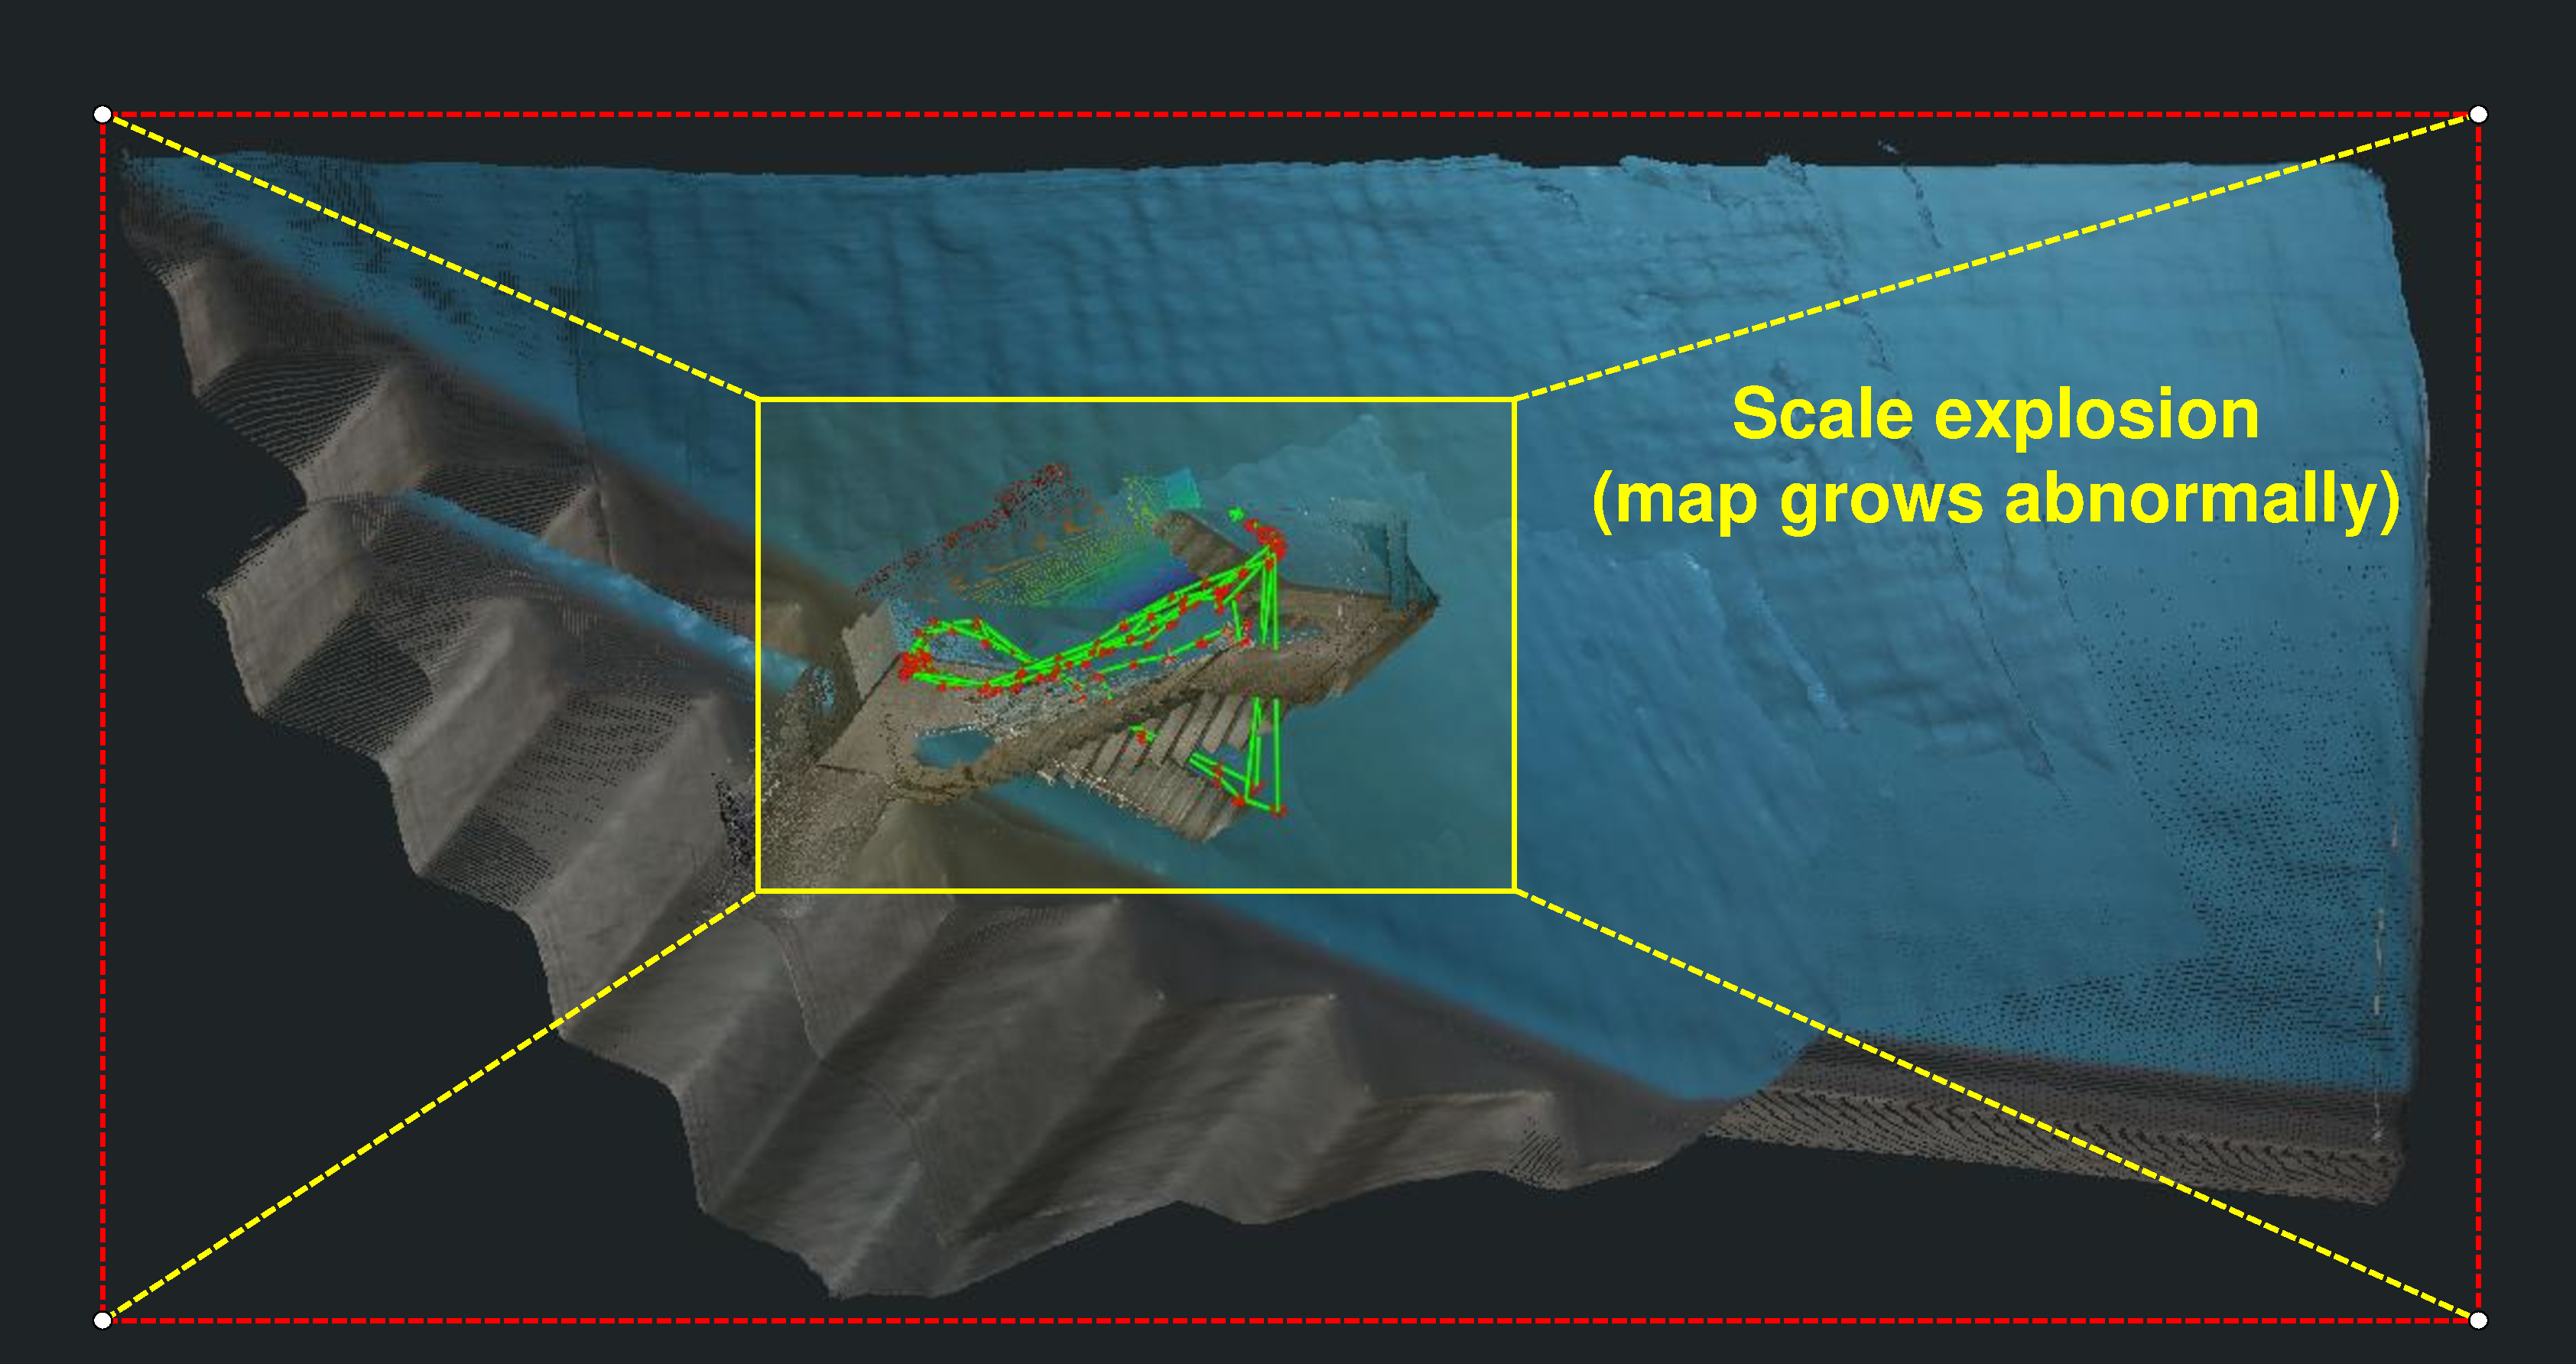
\includegraphics[width=0.98\columnwidth]{fig/fig1_resized.pdf}
    \caption{Representative example of scale inconsistency. During Sim(3) pose-graph optimization, the SLAM trajectory experiences a sudden scale explosion (highlighted), resulting in an abnormally enlarged reconstruction that diverges from the previously estimated map.}

    \vspace{-3mm}
    
    \label{fig:representative_figure}
\end{figure}

In this paper, we make the following key contributions:

\begin{itemize}

    \item \textbf{Systematic Analysis of Scale Inconsistencies:} We analyze how state-of-the-art monocular deep visual SLAM systems encounter \textbf{scale inconsistency} issues (as taxonomically analyzed in \figref{fig:problem_diagram}) in large-scale and complex indoor environments, highlighting vulnerabilities that are not fully revealed by existing benchmarks.
    
    \item \textbf{ScaleMaster Dataset and Baseline Evaluation:} We introduce the ScaleMaster Dataset, designed to examine scale consistency in challenging settings such as multi-floor structures, long trajectories, repetitive patterns, and low-texture areas. Using this dataset, we conduct baseline evaluations of representative deep-learning-based SLAM systems (DROID-SLAM \cite{teed2021droid}, MASt3R-SLAM \cite{murai2025mast3r}, VGGT-SLAM \cite{maggio2025vggt}), and reveal concrete cases of intra-session scale drift and inter-session scale ambiguity through both quantitative and qualitative analysis.
    
    \item \textbf{Complementary Use of Map Quality Metrics:} To address limitations of trajectory-only evaluation, we incorporate map-to-map metrics (Chamfer distance and Drop Rate), showing how they complement ATE by revealing distortions and scale collapse that remain hidden otherwise.
        
    
\end{itemize}


